%\setcounter{chapter}{1}
\chapter{Lăng kính}
\section{Lý thuyết trọng tâm}
\subsection{Cấu tạo lăng kính}
		\begin{center}
			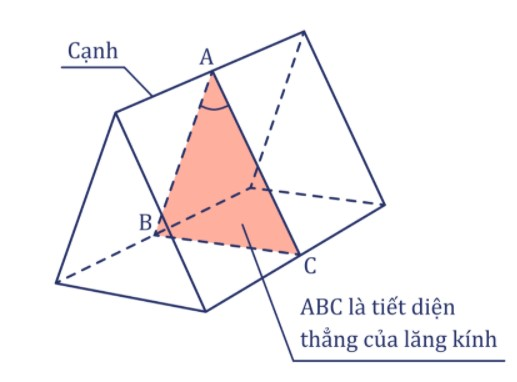
\includegraphics[scale=0.65]{../figs/VN11-PH-37-L-025-1-h2.jpg}
		\end{center}
	\begin{itemize}
		\item Lăng kính là một khối trong suốt, đồng chất(thủy tinh, nhựa,...), thường có dạng lăng trụ tam giác.
		\item Các phần tử của lăng kính gồm: cạnh, đáy, hai mặt bên.
		\item Về phương diện quang học, một lăng kính được đặc  trưng bởi góc chiết quang $A$ và chiết suất $n$.
			\end{itemize}

	\subsection{Đường truyền của tia sáng qua lăng kính}
	
\subsubsection{Tác dụng tán sắc của ánh sáng trắng}
	Lăng kính có tác dụng phân tích chùm ánh sáng trắng truyền qua nó thành nhiều chùm sáng màu khác nhau. Đó là sự tán sắc ánh sáng trắng qua lăng kính.
\subsubsection{Đường truyền của tia sáng qua lăng kính}
Chiếu đến mặt bên của lăng kính một chùm tia sáng hẹp đơn sắc SI như hình.
\begin{center}
	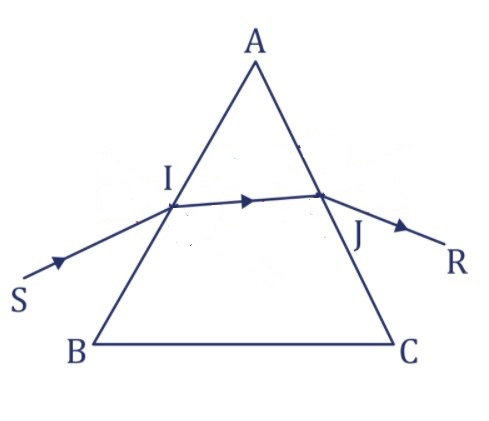
\includegraphics[scale=0.5]{../figs/VN11-PH-37-L-025-1-h3.jpg}
\end{center}
	
Góc tạo bởi tia ló và tia tới gọi là \textit{góc lệch $D$} của ánh sáng khi truyền qua lăng kính. 

\manatip{Nếu không xảy ra hiện tượng phản xạ toàn phần thì tia ló ra khỏi lăng kính bao giờ cũng bị lệch về phía đáy lăng kính.}	
\subsection{Công thức của lăng kính}
\begin{center}
	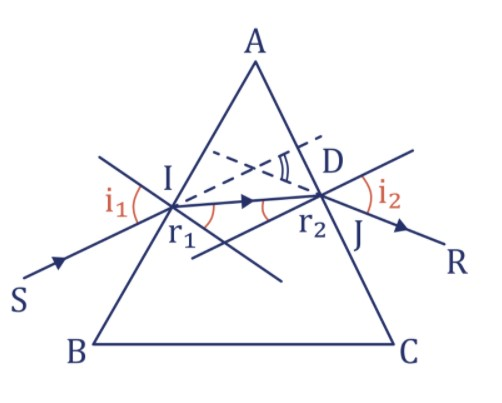
\includegraphics[scale=0.5]{../figs/VN11-PH-37-L-025-1-h1.jpg}
\end{center}
\begin{itemize}
\item Tại I: $sin i_1=n\sin r_1$.
\item Góc chiết quang: $A=r_1+r_2$.
\item Tại J: $sin i_2=n\sin r_2$.
\item Góc lệch của tia sáng qua lăng kính: $D=i_1+i_2-A$.
\end{itemize}
	
	\luuy{
		Nếu các góc nhỏ đều hơn $10^\circ$ thì các công thức trên được tính gần đúng là:
	\begin{itemize}
		\item $i_1=nr_1$,
		\item $A=r_1+r_2$,
		\item $i_2=nr_2$,
		\item $D=(n-1)A$.
	\end{itemize}
}

\subsection{Ứng dụng của lăng kính}
\subsubsection{Máy quang phổ}
Lăng kính là bộ phận chính của máy quang phổ.
\subsubsection{Lăng kính phản xạ toàn phần}
Lăng kính phản xạ toàn phần được sử dụng trong các ống nhòm, máy ảnh,...

\section{Bài tập}
\begin{dang}{Xác định các đại lượng liên quan đến lăng kính}
\end{dang}
\textbf{Phương pháp giải}

	
	Nếu các góc lớn hơn $10^\circ$, ta dùng công thức: 
	\begin{eqnarray*}
		\sin i_1&=&n\sin r_1,\\
		\sin i_2&=&n\sin r_2,\\
		A&=&r_1+r_2,\\
		D&=&i_1+i_2-A.
	\end{eqnarray*}	
	
	Nếu các góc nhỏ hơn $10^\circ$, ta mới được dùng công thức gần đúng sau: 
	\begin{eqnarray*}
	i_1&=&n r_1,\\
	i_2&=&n r_2,\\
	A&=&r_1+r_2,\\
	D&=&(n-1)A.
	\end{eqnarray*}	
	
	


\viduii{2}{	
Lăng kính có góc chiết quang $A=6^\circ$, chiết suất $n=\text{1,5}$. Góc lệch của tia sáng qua lăng kính bằng 
\begin{mcq}(4)
	\item $1^\circ$
	\item $3^\circ$.
	\item $6^\circ$.
	\item $12^\circ$.
\end{mcq}}{
\begin{center}
\textbf{Hướng dẫn giải}
\end{center}

{Vì góc chiết quang $A$ nhỏ hơn $10^\circ$, ta được dùng công thức gần đúng sau:
	
 $D=(n-1)A=\left(\text{1,5}-1 \right) \cdot 6^\circ=3^\circ$.

	
Góc lệch của tia sáng qua lăng kính bằng $\text{3}^\circ$.
	
	\textbf{Đáp án: B.}
}}

\viduii{3}{
	Lăng kính có góc chiết quang $A=30^\circ$, chiết suất $n=\text{1,5}$. Chiếu vào mặt bên của lăng kính một tia sáng có góc tới $i=40^\circ$. Góc lệch của tia sáng qua lăng kính gần bằng 
	\begin{mcq}(4)
		\item $15^\circ$
		\item $17^\circ$.
		\item $19^\circ$.
		\item $21^\circ$.
	\end{mcq}}
{
	\begin{center}
		\textbf{Hướng dẫn giải:}
	\end{center}
	
	{Áp dụng công thức: $\sin i_1=n\sin r_1$
		
		Với $i_1=40^\circ,\ n=\text{1,5} $. Ta tìm được $r_1=\text{25,37}^\circ$.
		
		Áp dụng công thức: $A=r_1+r_2$
		
		Với $r_1=\text{25,37}^\circ,\ A=30^\circ$. Ta tìm được $r_2=\text{4,62}^\circ$.
		
		Áp dụng công thức: $\sin i_2=n\sin r_2$
		
		Với $r_2=\text{4,62}^\circ,\ n=\text{1,5} $. Ta tìm được $i_2\approx \text{17}^\circ$.
		
	Góc lệch của tia sáng qua lăng kính gần bằng $\text{17}^\circ$.
		
		\textbf{Đáp án: B.}
		
		
	}}

\viduii{3}{
Một lăng kính có góc chiết quang $A$. Chiếu tia sáng $SI$ đến vuông góc với mặt bên của lăng kính. Biết góc lệch của tia ló và tia tới là $D=15^\circ$. Cho biết chiết suất của lăng kính là $n=\dfrac{4}{3}$. Góc chiết quang $A$ gần bằng

\begin{mcq}(4)
	\item $34^\circ$
	\item $35^\circ$.
	\item $36^\circ$.
	\item $37^\circ$.
\end{mcq}}
{
\begin{center}
	\textbf{Hướng dẫn giải:}
\end{center}

 Vì tia sáng tới vuông góc với mặt bên nên $i_1=0^\circ \Rightarrow A=r_1+r_2=r_2$.
	
	Mà $D=i_1+i_2-A=15^\circ \Rightarrow i_2=15^\circ+A$.
	
	$\sin i_2=n\sin r_2 \Rightarrow \sin\left( 15^\circ+A\right)=\text{1,5}\sin A \Rightarrow \sin 15^\circ\cdot \cos A+\cos 15^\circ\cdot \sin A$.
	
	$\Rightarrow \tan A=\dfrac{\sin 15^\circ}{\left( \dfrac{4}{3}-\cos15^\circ \right) }=\text{0,7044}\approx 36^\circ$.
	
\textbf{	Đáp án: C.}
	
	
}

\viduii{3}{

Một lăng kính có thiết diện thẳng là tam giác đều ABC. Chiếu tia sáng SI đến vuông góc với mặt bên AB của lăng kính với góc tới là $30^\circ$ thì tia ló ra khỏi không khí rà sát mặt AC của lăng kính. Tính chiết suất của chất làm lăng kính. 

\begin{mcq}(4)
	\item $\text{1,33}$.
	\item $\text{1,42}$.
	\item $\text{1,527}$.
	\item $\text{1,71}$.
\end{mcq}
}{
\begin{center}
	\textbf{Hướng dẫn giải:}
\end{center}

{ 
	Vì tia ló đi ra khỏi không khí ra sắt mặt AC của lăng kính nên $i_2=90^\circ$.
	
	Ta có: $\sin i_1=n\sin r_1,\ \sin i_2=n\sin r_2$.
	
	$\Rightarrow \dfrac{\sin i_1}{\sin i_2}=\dfrac{\sin r_1}{\sin r_2}$
	
	 $\Leftrightarrow \dfrac{\sin i_1}{\sin i_2}=\dfrac{\sin r_1}{\sin \left( 60^\circ-r_1\right) }$.
	 
	 $\Rightarrow r_1=\text{19,1}^\circ$.
	 
	 $\Rightarrow n= \dfrac{\sin i_1}{\sin r_1}=\text{1,527}$.
	 
		
\textbf{Đáp án: C.}
	
	
}
}	


